\documentclass[10pt]{article}
\usepackage[ngerman]{babel}
\usepackage[utf8]{inputenc}
\usepackage[T1]{fontenc}
\usepackage{amsmath}
\usepackage{amsfonts}
\usepackage{amssymb}
\usepackage[version=4]{mhchem}
\usepackage{stmaryrd}
\usepackage{graphicx}
\usepackage[export]{adjustbox}
\graphicspath{ {./images/} }

\title{Hauptprüfung Abiturprüfung 2024 - Leistungsfach }

\author{Alexander Schwarz\\
www.mathe-aufgaben.com}
\date{}


\begin{document}
\maketitle
 Baden-Württemberg

\section*{Aufgabe III 1}
Ein bekannter Video-Streamingdienst bietet einen kostenpflichtigen Zugang zu Spielfilmen und Serien an. Personen, die davon gegen Zahlung einer monatlichen Gebühr Gebrauch machen, werden im Folgenden als Abonnenten bezeichnet. Sie haben sich entweder für das Spielfilmpaket oder für das Komplettpaket entschieden, das neben den Spielfilmen auch noch Serien enthält.

Unter den Abonnenten sind 70\% höchstens 40 Jahre alt. Von diesen haben 80\% das Komplettpaket gewählt. Unter denjenigen Abonnenten, die älter als 40 Jahre sind, haben sich $50 \%$ für das Komplettpaket entschieden.\\
a) Stellen Sie den Sachverhalt in einem beschrifteten Baumdiagramm dar.\\
b) Eine unter allen Abonnenten zufällig ausgewählte Person hat sich für das Komplettpaket entschieden. Bestimmen Sie die Wahrscheinlichkeit dafür, dass sie höchstens 40 Jahre alt ist.\\
c) Bestimmen Sie die Anzahl der Abonnenten, die man mindestens zufällig auswählen müsste, damit unter innen mit einer Wahrscheinlichkeit von mindestens $99 \%$ mehr als fünf Personen älter als 40 Jahre sind.

Der Anteil der zufriedenen Abonnenten von derzeit 60\% soll gesteigert werden. Dazu wird ein Algorithmus entwickelt, der jedem Abonnenten täglich individuell einen Spielfilm vorschlägt. Als Basis für die Entscheidung über den dauerhaften Einsatz des Algorithmus plant das Management einen Probebetrieb. Im Anschluss soll die Nullhypothese „Der Anteil der zufriedenen Abonnenten beträgt höchstens 60\%." mithilfe einer Stichprobe von 200 zufällig ausgewählten Abonnenten auf einem Signifikanzniveau von 5\% getestet werden.\\
d) Geben Sie an, welche Überlegung des Managements zur Wahl dieser Nullhypothese geführt haben könnte.

Für den beschriebenen Test ergibt sich \{132; 133; ...;200\} als der Ablehnungsbereich der Nullhypothese.\\
e) Zur Bestimmung der unteren Grenze dieses Ablehnungsbereichs wurden zunächst folgende Lösungsschritte ausgeführt:

\begin{itemize}
  \item Y: Anzahl der zufriedenen Abonnenten in der Stichprobe
  \item $P_{0,6}^{200}(Y \geq 132) \approx 0,047$
\end{itemize}

Begründen Sie, dass die beiden Lösungsschritte zur Bestimmung der unteren Grenze nicht ausreichend sind, und ergänzen Sie diese geeignet. (4 BE)\\
f) Weisen Sie nach, dass die Wahrscheinlichkeit für einen Fehler zweiter Art bei diesem Ablehnungsbereich der Nullhypothese mehr als 90\% betragen könnte.

Zur Anmeldung auf der Webseite des Streamingdiensts ist ein persönliches Kennwort erforderlich. Für das Kennwort können 80 verschiedene Zeichen verwendet werden: je 26 Groß- und Kleinbuchstaben, 10 Ziffern sowie 18 Sonderzeichen.\\
g) Einige Abonnenten verwenden ein Kennwort, das genau acht Zeichen lang ist und nur aus Kleinbuchstaben besteht. Dabei können Zeichen mehrfach vorkommen. Zeigen Sie, dass für diese Abonnenten weniger als ein Tausendstel aller möglichen Kennwörter infrage kommen, die aus genau acht Zeichen bestehen.\\
h) Niclas beschließt ein Kennwort zu wählen, das die beiden folgenden Bedingungen erfüllt:

\begin{itemize}
  \item Es besteht aus genau acht Zeichen, die untereinander verschieden sind.
  \item Die Buchstaben seines Namens sind in der korrekten Reihenfolge und unter Berücksichtigung der Groß- und Kleinschreibung enthalten.
\end{itemize}

Damit sind beispielsweise Nic4+las oder nNicl*as mögliche Kennwörter. Bestimmen Sie die Anzahl aller derartigen Kennwörter.\\
(3 BE)

\section*{Aufgabe III 1}
a) A: „Ein Abonnent ist höchstens 40 Jahre alt."

B: „Ein Abonnent hat das Komplettpaket."\\
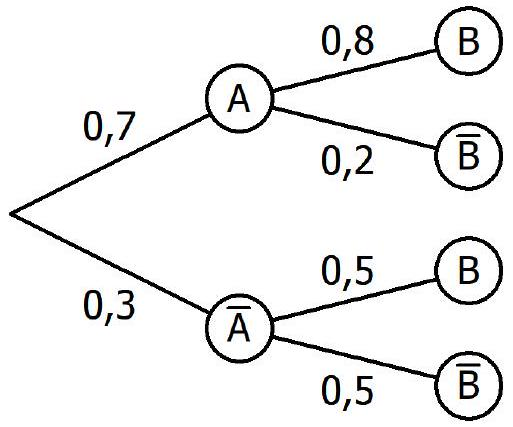
\includegraphics[max width=\textwidth, center]{2025_04_24_3da0d7028731b4368807g-4}\\
b) Es handelt sich um eine bedingte Wahrscheinlichkeit:\\
$P_{B}(A)=\frac{P(A \cap B)}{P(B)}=\frac{0,7 \cdot 0,8}{0,7 \cdot 0,8+0,3 \cdot 0,5} \approx 0,79$\\
c) Die Zufallsgröße X zählt die Abonnenten, die älter als 40 Jahre sind.

X ist binomialverteilt mit unbekanntem n und $\mathrm{p}=0,3$.\\
Bedingung: $P(X>5) \geq 0,99$

$$
\begin{aligned}
& \Leftrightarrow 1-P(X \leq 5) \geq 0,99 \\
& \Leftrightarrow P(X \leq 5) \leq 0,01
\end{aligned}
$$

Probe mit WTR: $n=39: P(X \leq 5) \approx 0,011$

$$
\mathrm{n}=40: \mathrm{P}(\mathrm{X} \leq 5) \approx 0,009
$$

Es müssen mindestens 40 Personen ausgewählt werden.\\
d) Nullhypothese: „Der Anteil der zufriedenen Abonnenten beträgt höchstens 60\%." Gegenhypothese: „Der Anteil der zufriedenen Abonnenten beträgt mehr als 60\%."

Das Management möchte den Fehler 1.Art auf eine Wahrscheinlichkeit von maximal 5\% (Signifikanzniveau) beschränken.\\
Ein Fehler 1.Art tritt ein, wenn der Test zum Ergebnis kommt, dass der Anteil mehr als 60\% beträgt, der Anteil in Wahrheit aber höchstens 60\% beträgt. Es soll also vermieden werden, den Algorithmus dauerhaft einzusetzen, obwohl der Einsatz des Algorithmus die Zufriedenheit unter den Abonnenten nicht erhöht.\\
e) Durch die Bedingung $P_{0,6}^{200}(Y \geq 132) \approx 0,047$ ist nicht gewährleistet, dass es auch eine natürliche Zahl $k$ mit $k<132$ geben könnte, für die ebenfalls gilt: $P_{0,6}^{200}(Y \geq k) \leq 0,05$.

Geeignete Ergänzung:\\
Es gilt $P_{0,6}^{200}(Y \geq 131)=1-P_{0,6}^{200}(Y \leq 130) \approx 0,064$\\
Damit ist 132 die untere Grenze des Ablehnungsbereichs.\\
f) Eine hohe Wahrscheinlichkeit für einen Fehler 2.Art tritt auf, wenn die Trefferwahrscheinlichkeit p > 0,6 beträgt, jedoch nicht sehr weit von 0,6 entfernt liegt.

Wähle z.B. p = 0,61, das heißt der Anteil der zufriedenen Abonnenten beträgt tatsächlich 61\%.\\
$P($ Fehler 2.Art $)=P_{0,6}^{200}(Y \leq 131) \approx 0,917$\\
Hinweis: $Y \leq 131$ ist erforderlich, da $Y$ bei einem Fehler 2.Art außerhalb des Ablehnungsbereiches liegen muss.\\
g) Anzahl aller 8-stelligen Passwörter, die nur aus Kleinbuchstaben bestehen: $26^{8}$ Anzahl aller möglichen 8-stelligen Passwörter: $80^{8}$

Anteil: $\frac{26^{8}}{80^{8}} \approx 0,00012<\frac{1}{1000}$ was zu zeigen war\\
h) Da „Niclas" 6 Buchstaben besitzt, bleiben für die beiden anderen Stellen noch 74 bzw. 73 Möglichkeiten übrig.

Die beiden anderen Stellen können an zwei beliebigen der insgesamt 8 Plätze stehen. Hierfür gibt es insgesamt $\binom{8}{2}$ Möglichkeiten zur Platzierung.

Die Gesamtanzahl der Möglichkeiten beträgt daher $74 \cdot 73 \cdot\binom{8}{2}=151256$.


\end{document}